\section{QR Decomposition Implementation}

\subsection{CPU Implementation}
The standard algorithm for the QR decomposition involves successive Householder transformations [BOOK QUOTE]. To implement QR decomposition on the CPU, we followed the outline of the algorithm in [BOOK] almost exactly. 
In the book's implementation, the Householder algorithm runs on all columns except for the last one. We modified the implementation such that the last column is also transformed with the Householder method. By doing this we do not have to handle a special case separately. 
Our implementation of the algorithm can be seen in [APPENDIX LISTING]. 
\\\\
We have a limited understanding of the underlying math behind QR decomposition, but the general flow of the algorithm is as follows:

\begin{enumerate}
    \item Each column of the matrix is considered one at a time. In iteration k, only elements from the kth element and below are considered. 
    \item For numerical stability purposes, all elements will temporarily be scaled down by the maximal entry of the column. 
    \item If all the entries of a column are zero, then the matrix is determined to be singular. 
    \item The diagonal length of the hyperplane with k dimensions is determined by calculating the square root of the sum of the squares of the each entry of the kth column. 
    \item The inner product for the remaining square matrix with dimension k is computed to transform itself. 

\end{enumerate}

\begin{lstlisting}[language=C, caption={QR Decomposition on the CPU}, label={lst:qr_decomposition_cpu}]
// returns true if the matrix is singular
bool matrix_qr_decomposition(matrix_t *matrix, float *diagonal, float *c) {
    float column_length;  // sigma in book
    float column_length_squared, element;
    int n = matrix->columns;
    float scale;
    bool is_singular = false;
    // for every column
    for (int k = 0; k < n; k++) {
        scale = 0.0f;
        // scale is the max absolute value of the column
        for (int i = k; i < n; i++)
            scale = fmaxf(scale, fabsf(matrix->values[INDEX(i, k, n)]));

        if (scale == 0.0) {
            is_singular = true;
            c[k] = diagonal[k] = 0.0f;
            continue;
        }
        // Normalize column
        for (int i = k; i < n; i++) matrix->values[INDEX(i, k, n)] /= scale;

        // column length below diagonal
        column_length_squared = 0.0f;  // sum in book.
        for (int i = k; i < n; i++) {
            element = matrix->values[INDEX(i, k, n)];
            column_length_squared += element * element;
        }

        // column length below diagonal, with the sign of diagonal k
        column_length =
            SIGN(sqrtf(column_length_squared), matrix->values[INDEX(k, k, n)]);

        // add column length to diagonal k
        matrix->values[INDEX(k, k, n)] += column_length;

        c[k] = matrix->values[INDEX(k, k, n)] * column_length;

        diagonal[k] = -scale * column_length;

        // Calculate Q[k] = I - (u[k] (x) u[k]) / c[k]
        for (int j = k + 1; j < n; j++) {
            // inner product for column j below diagonal
            float inner_product = 0.0f;
            for (int i = k; i < n; i++) {
                inner_product += matrix->values[(INDEX(i, k, n))] *
                                 matrix->values[(INDEX(i, j, n))];
            }

            // division
            float tau = inner_product / c[k];

            for (int i = k; i < n; i++) {
                matrix->values[(INDEX(i, j, n))] -=
                    tau * matrix->values[(INDEX(i, k, n))];
            }
        }
    }

    if (!is_singular) is_singular = diagonal[n - 1] == 0.0f;
    return is_singular;
}
\end{lstlisting}

\subsection{GPU Implementation} 

To optimize the performance of QR decomposition with GPU accelerated code, we firstly factored out the parts the can run independently. This includes scaling every element of a column by a factor and subtracting a certain value from every element of a column. These were implemented in the same way as our fastest matrix addition implementation, where each block and thread is responsible for transforming a subset of the elements. 

\subsubsection{Parallel Reduction}
A more interesting problem to solve in parallel is what we have classified reduction algorithms. Reduction algorithms are defined as computing an accumulation of elements by some associative operation. In our case we had to find the maximal absolute element of a column as well as finding the sum of a column. [REFERENCE TO PARALLEL MAX]
This algorithm was inspired by (LINK: https://ernie55ernie.github.io/parallel%20programming/2018/03/17/cuda-maximum-value-with-parallel-reduction.html) 

The algorithm works by operating on pairs of elements in a tree-like structure until only one element is left. 

\begin{figure}[ht]
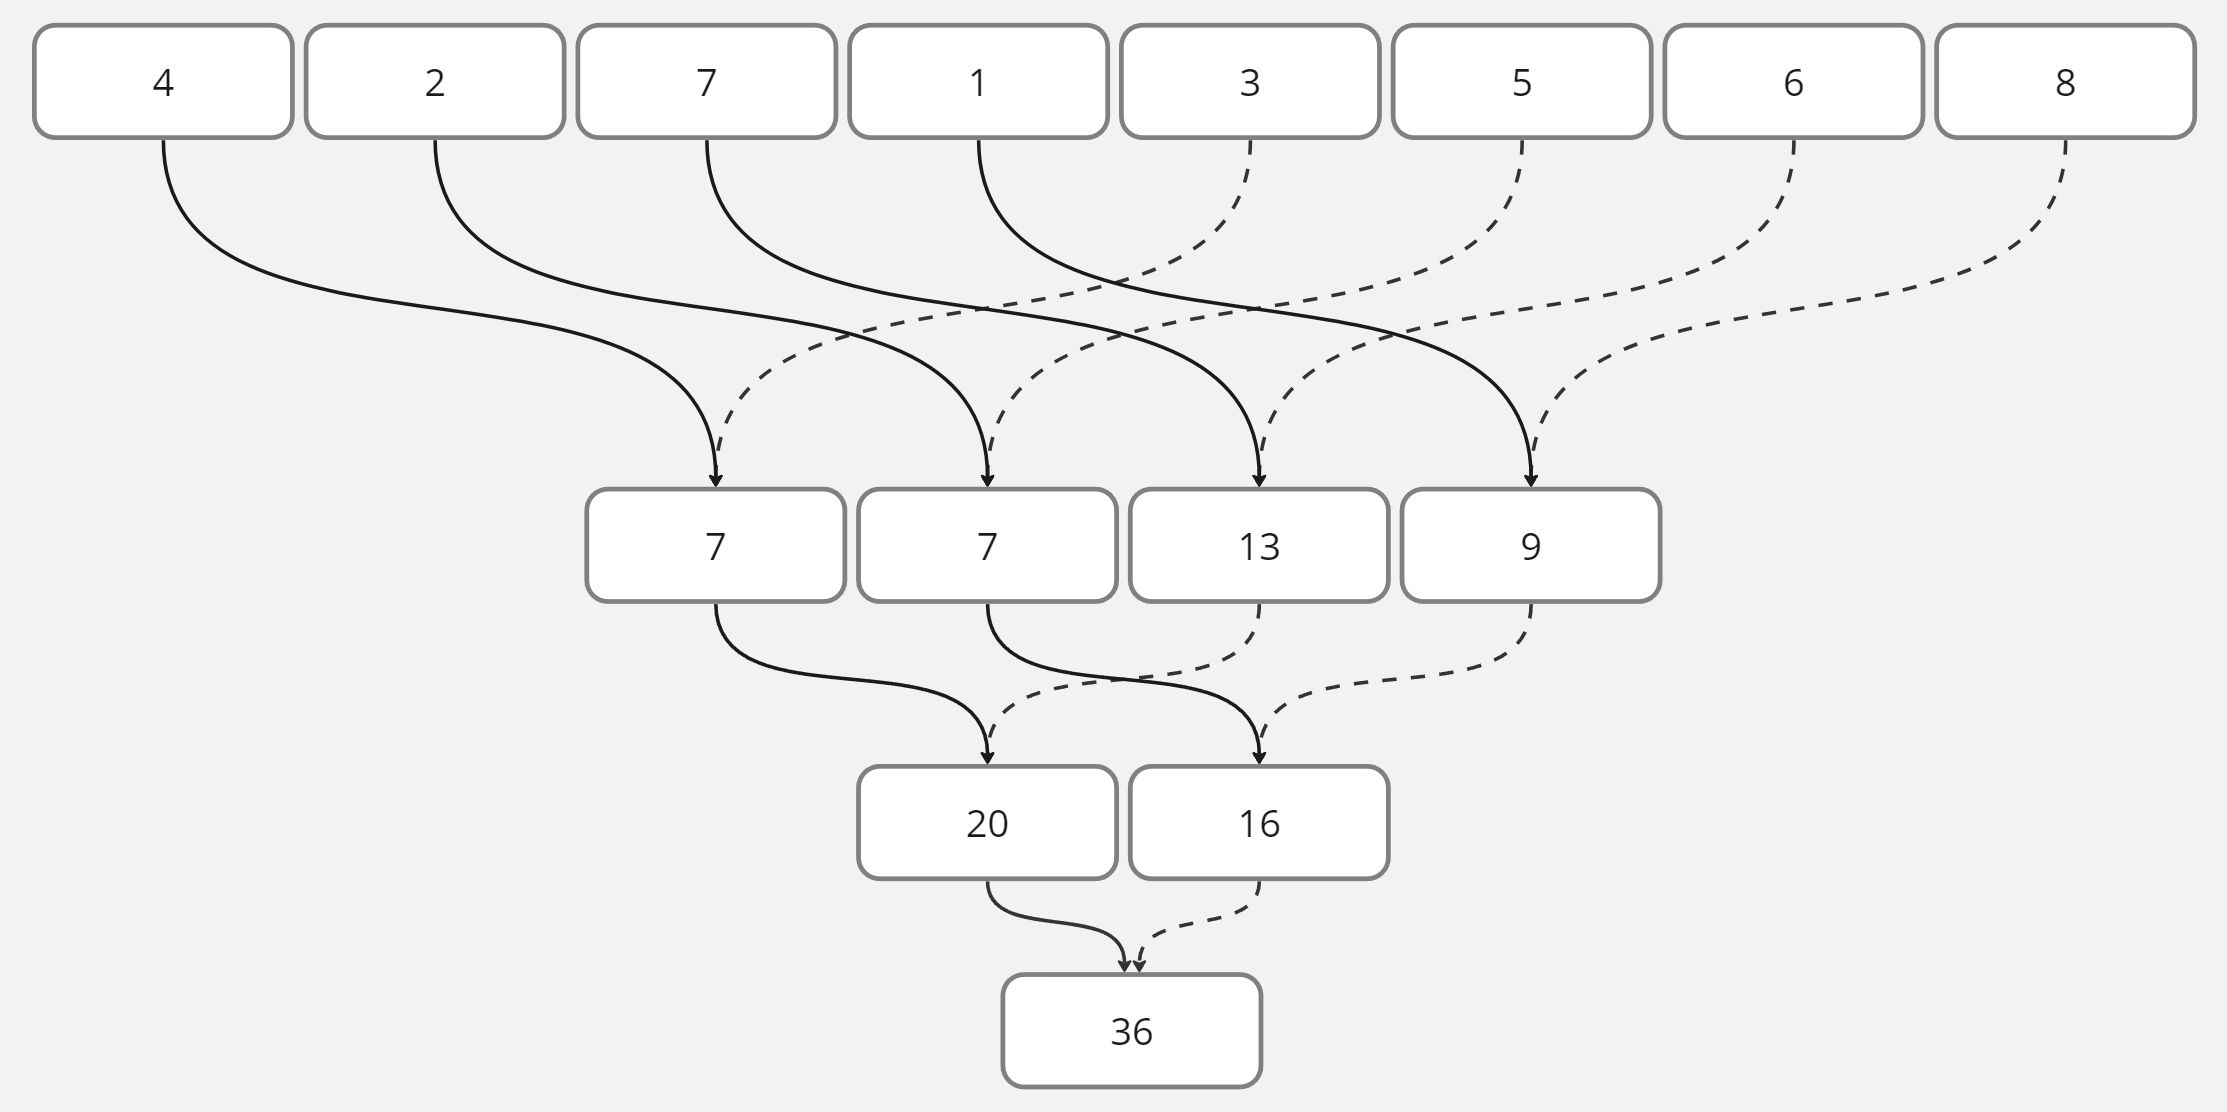
\includegraphics[width=\textwidth]{Documents/Report/Figures/parallel_sum.png}
\caption{Example of summation by parallel reduction.}
\label{fig:threads and blocks}
\end{figure}

Our implementation can be seen in the code below. Please note that our algorithm is generalized such that we can pass any associative function pointer as the reducer. \\
The algorithm works by distributing the responsibility of each entry in the list to a thread. The $split\_index$ variable keeps track of the middle of the remaining elements to be paired up. This variable also acts as an offset, to calculate which element a given entry should be paired up with. On each iteration element$_k$ is paired up with element$_{k + split\_index}$ and stored in element$_k$. After each iteration, the $split\_index$ is halved. To prevent us from accessing out of bounds, a predicate checks if $k < split\_index$. To prevent race conditions, we synchronize all threads before starting the next iteration. 

\begin{lstlisting}[language=C, caption={Parallel Reduction}, label={lst:parallel_reduce}]
typedef float (*reducer_t)(float, float);

__device__ void cuda_parallel_reduction(
    float *cache, int cache_index, reducer_t reduce) {
    int split_index = blockDim.x;
    while (split_index != 0) {
        split_index /= 2;
        if (cache_index < split_index)
            cache[cache_index] =
                reduce(cache[cache_index], cache[cache_index + split_index]);

        __syncthreads();
    }
}
\end{lstlisting}

\subsection*{Final Details}
In our final implementation of a GPU QR decomposition, we utilize a CPU runner responsible for launching kernels. Each kernel is launched with an appropriate amount of threads and blocks depending on the work required. Each column must still sequentially go through the Householder method, thus preventing us from running the algorithm completely in parallel. This runner is also responsible for allocating, copying and freeing memory related to the GPU. 